\documentclass[tikz,border=2pt]{standalone}
\usepackage{tikz}
\usepackage[european]{circuitikz}
\usetikzlibrary{arrows.meta,positioning,calc}
../cictikz/src/cictikz/data/tex/cictikz_lib.tex
\begin{document}
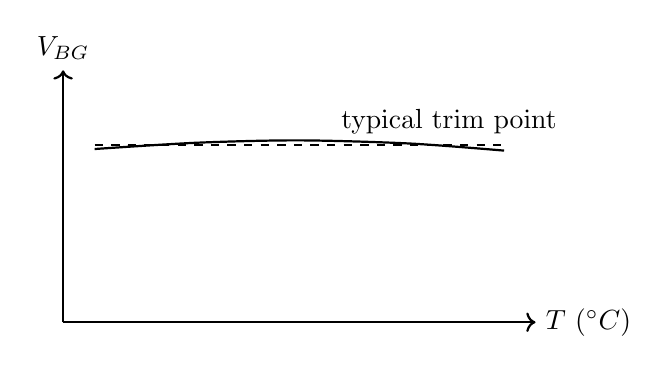
\begin{tikzpicture}[line width=0.8pt]
  \draw[->] (0,0) -- (6,0) node[right] {$T\ (^\circ C)$};
  \draw[->] (0,0) -- (0,3.2) node[above] {$V_{BG}$};
  \draw[smooth] plot coordinates {(0.4,2.2) (1.7,2.28) (3.0,2.31) (4.4,2.27) (5.6,2.18)};
  \draw[dashed] (0.4,2.25) -- (5.6,2.25);
  \node at (4.9,2.55) {typical trim point};
\end{tikzpicture}
\end{document}
